\subsection{The fish shoal}

\begin{figure}
\centering
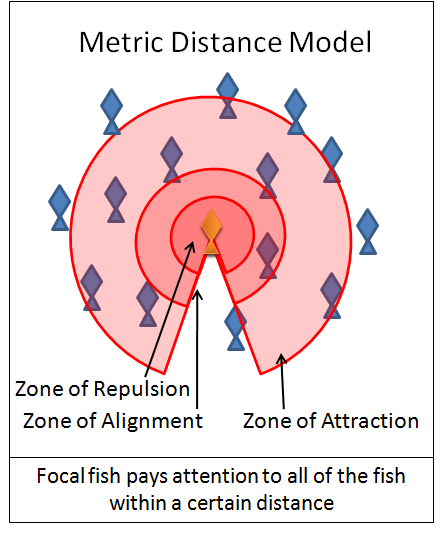
\includegraphics[width=0.45\textwidth]{figs/swarmfig.png}
\caption{\label{fig:swarm} Fish shoal model.}
\end{figure}

The swarming model used is based on the two models found in the references \cite{javafish} and \cite{matlabfish}. It follows the same rules as the basic swarming model, namely repulsion, alignment and attraction. Each of these rules applies at a certain distance range from the fish which can be seen in figure \ref{fig:swarm}. If another fish enters the zone of repulsion they will tend to repel each other and not surprisingly if they are within the attraction distance, they will tend to move towards each other. In the zone of alignment they tend to align themselves so that they will move in the same direction as the other fishes in that zone. Behind the fish there is also a dead zone where no interaction occur (most animals can not see things behind themselves). To further improve the behavior of the swarm, there is also an addition to the algorithm called distance priority \cite{matlabfish}. It makes the fish tend to align itself to the average direction of a set number of its closest neighbors, regardless of which zone they are in.\\
\\
The fishes in the shoal move at a constant drift speed but can accelerate to a max speed to avoid the shark. The way the fishes in this model avoids the shark is quite simple. A scare distance is set for the fishes and should the predator be within this distance, the fish will completely ignore the swarming rules and update the velocity according to
\begin{equation}
\vec{v}_f \rightarrow \vec{v}_f - (\vec{x}_s - \vec{x}_f)a
\end{equation}
where $\vec{v}_f$ is the velocity of the fish, $\vec{x}_s$ the position of the shark, $\vec{x}_f$ the position of the fish and $a$ is a constant called acceleration rate, which decides how fast the fish will be able to reach its max speed (note that the time step is excluded since it will always be set to 1). In other words the fish will just move in opposite direction of where the shark is relative to itself starting at its drift speed and accelerating to its max speed. Having the avoidance rule this way makes for a problem however since this could force a fish to move outside of the attraction zone of the fishes furthest out in the shoal. To solve this it is added that should a fish get too far away from the center of the shoal (average position of all fishes), it will move strictly towards this point if not too close to the shark.


